\begin{minipage}{0.49\textwidth}
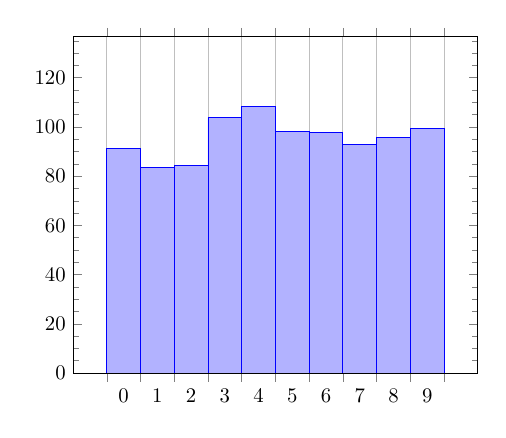
\begin{tikzpicture}[scale=0.75]
  \begin{axis}[ybar interval, ymax=136.628,ymin=0, minor y tick num = 3]
    \addplot coordinates { (0,91.1241) (1,83.3379) (2,84.3466) (3,103.738) (4,108.462) (5,97.9569) (6,97.8569) (7,92.7793) (8,95.5845) (9,99.3431) (10, 62.1034) };
  \end{axis}
\end{tikzpicture}
\caption*{Average weights repartitions on several trees}
\end{minipage}
\begin{minipage}{0.49\textwidth}
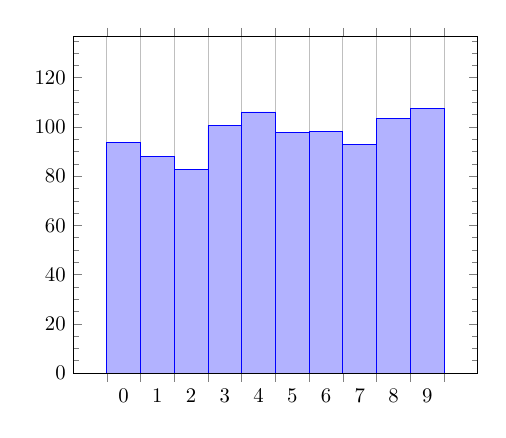
\begin{tikzpicture}[scale=0.75]
  \begin{axis}[ybar interval, ymax=136.628,ymin=0, minor y tick num = 3]
    \addplot coordinates { (0,93.7586) (1,87.8966) (2,82.5517) (3,100.466) (4,106.069) (5,97.8448) (6,98.1724) (7,93.0345) (8,103.345) (9,107.569) (10, 62.1034) };
  \end{axis}
\end{tikzpicture}
\caption*{Average weights repartitions on one of the trees}
\end{minipage}
\begin{minipage}{0.49\textwidth}
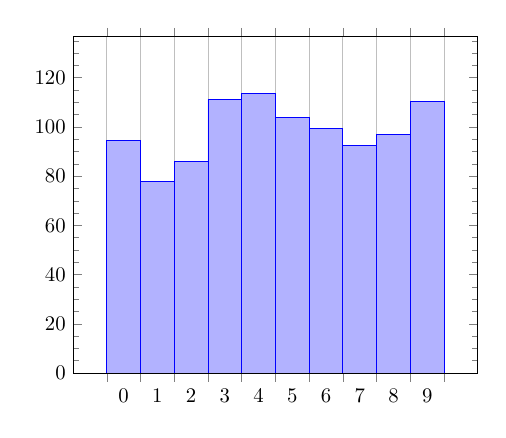
\begin{tikzpicture}[scale=0.75]
  \begin{axis}[ybar interval, ymax=136.628,ymin=0, minor y tick num = 3]
    \addplot coordinates { (0,94.3103) (1,77.8793) (2,85.9828) (3,111.19) (4,113.534) (5,103.672) (6,99.2931) (7,92.5345) (8,97) (9,110.241) (10, 62.1034) };
  \end{axis}
\end{tikzpicture}
\caption*{Average weights repartitions on one of the trees}
\end{minipage}
\begin{minipage}{0.49\textwidth}
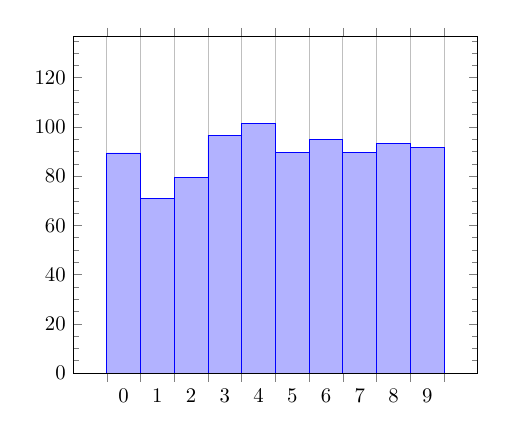
\begin{tikzpicture}[scale=0.75]
  \begin{axis}[ybar interval, ymax=136.628,ymin=0, minor y tick num = 3]
    \addplot coordinates { (0,89.3966) (1,71) (2,79.6034) (3,96.6034) (4,101.276) (5,89.6034) (6,94.7931) (7,89.7069) (8,93.3793) (9,91.6724) (10, 62.1034) };
  \end{axis}
\end{tikzpicture}
\caption*{Average weights repartitions on one of the trees}
\end{minipage}
